
\lecture{14}{Engines and Refrigerators}{Qiang Zhu}{scribe-name1,2,3}



\section{Real Heat Engines}
In the previous lecture, we have learned the theoretical limit of heat engines.
It is useful to know the upper limit when we design an engine.
However, one might also ask how it work in reality.
Can we follow the Carnot cycle in practice?

Now, let's discuss a few of the engines used in the real world.

\begin{figure}[ht]
\centering
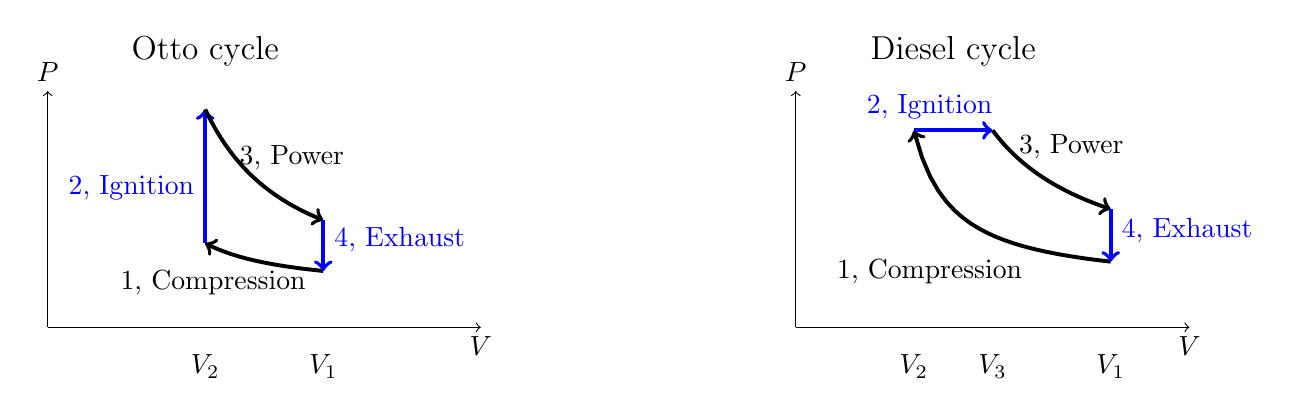
\begin{tikzpicture} %[x=8cm, y=4cm]
\draw [->] (-0.5, -0.5) -- (5.0,-0.5) node[below]{$V$};
\draw [->] (-0.5, -0.5) -- (-0.5, 2.5)  node[above]{$P$};
\draw [->, line width=0.05cm, black,domain=3.0:1.5]  plot(\x, {1/((\x)^(1.4))}) node[below, xshift=0.1cm, yshift=-0.2cm] {1, Compression};
\draw [->, line width=0.05cm, blue] (1.5,0.567) -- (1.5,2.267)  node[left, yshift=-1cm]                                  {2, Ignition};
\draw [->, line width=0.05cm, black,domain=1.5:3.0]  plot(\x, {4/((\x)^(1.4))}) node[above, xshift=-0.4cm, yshift=0.5cm] {3, Power};
\draw [->, line width=0.05cm, blue] (3.0,0.859) -- (3.0,0.215)  node[right, yshift=0.4cm]                                {4, Exhaust};
\node at (1.5, -1) {$V_2$};
\node at (3.0, -1) {$V_1$};
\node  at (1.5, 3) {\large Otto cycle};

\draw [->] (9.0,-0.5) -- (14.0, -0.5) node[below]{$V$};
\draw [->] (9.0,-0.5) -- ( 9.0, 2.5) node[above]{$P$};
\draw [->, line width=0.05cm, black,domain=13.0:10.5]  plot(\x, {1/(\x-10)}) node[below, xshift=0.2cm, yshift=-1.5cm] {1, Compression};
\draw [->, line width=0.05cm, blue] (10.5,2.0) -- (11.5,2.0)  node[above, xshift=-0.8cm]                              {2, Ignition};
\draw [->, line width=0.05cm, black,domain=11.5:13.0]  plot(\x, {3/(\x-10)}) node[above, xshift=-0.5cm, yshift=0.5cm] {3, Power};
\draw [->, line width=0.05cm, blue] (13.0,1.0) -- (13.0,0.333)  node[right, yshift=0.4cm]                             {4, Exhaust};
\node at (10.5, -1) {$V_2$};
\node at (11.5, -1) {$V_3$};
\node at (13.0, -1) {$V_1$};
\node at (11.0, 3) {\large Diesel cycle};
\end{tikzpicture}
\caption{The Otto cycle and Diesel cycle.}
\end{figure}

Recalling what we learned about P-V diagrams in compression work, we can trivially derive the efficiency as a function of $V$
\begin{equation}
PV^{\gamma} = \text{const} ~~~~\rightarrow~~~~~~ e = 1-(\frac{V_2}{V_1})^{\gamma-1} 
                                                   = 1-\frac{T_1}{T_2} 
                                                   = 1-\frac{T_3}{T_4}~~~~~~~~~~~~~ \text{(Otto cycle)}
\end{equation}
\begin{equation}
PV = \text{const} ~~~~\rightarrow~~~~~~ e = 1-\frac{V_2}{V_1}  ~~~~~~~~~~~~~ \text{(Diesel cycle)}
\end{equation}
\\
\begin{figure}[ht]
\centering
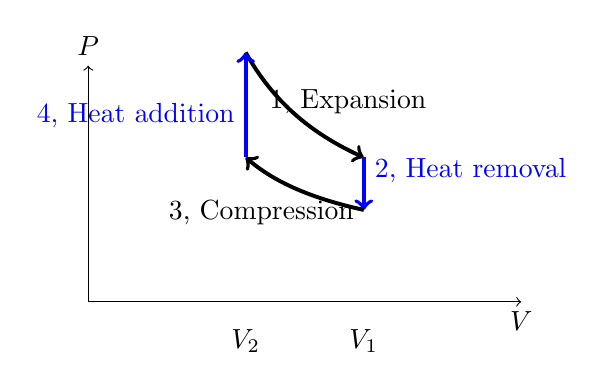
\begin{tikzpicture} %[x=8cm, y=4cm]
\draw [->] (-0.5, -0.5) -- (5.0,-0.5) node[below]{$V$};
\draw [->] (-0.5, -0.5) -- (-0.5, 2.5)  node[above]{$P$};
\draw [->, line width=0.05cm, black,domain=1.5:3.0] plot(\x, {4/\x}) node[below, xshift=-0.2cm, yshift=1cm] {1, Expansion};
\draw [->, line width=0.05cm, blue] (3.0,1.333) -- (3.0,0.667)  node[right, yshift=0.5cm]                    {2, Heat removal};
\draw [->, line width=0.05cm, black,domain=3.0:1.5] plot(\x, {2/\x}) node[above, xshift=0.2cm, yshift=-1cm] {3, Compression};
\draw [->, line width=0.05cm, blue] (1.5,1.3333) --(1.5,2.667)  node[left, yshift=-0.8cm]                   {4, Heat addition};
\node at (1.5, -1) {$V_2$};
\node at (3.0, -1) {$V_1$};
\end{tikzpicture}
\caption{The idealized Stirling cycle.}
\end{figure}



Discussion on Stirling Engines
\\\\\\\\\\\\\\\\\\\\\\\\
\section{Steam Engines and Real Refrigerators}
A very different type of engine is the steam engine, in which the liquid water/steam is used as the work substance. It works as follows,
\begin{enumerate}
\item water is pumped to high pressure at nearly constant volume;
\item water flows into a boiler at constant pressure, then becomes steam;
\item steam hits the turbine, where it expands adiabatically, cools, the ends up at the original pressure;
\item the fluid is cooled further to become water.
\end{enumerate}

On the other hand, a refrigerator works as follows,
\begin{enumerate}
\item gas is compressed to adiabatically;
\item gives up heat and become liquid at constant pressure;
\item passes through a throttling valve to 
\item absorbs heat and turns back to a gas in the evaporator
\end{enumerate}
\begin{figure}[ht]
\centering
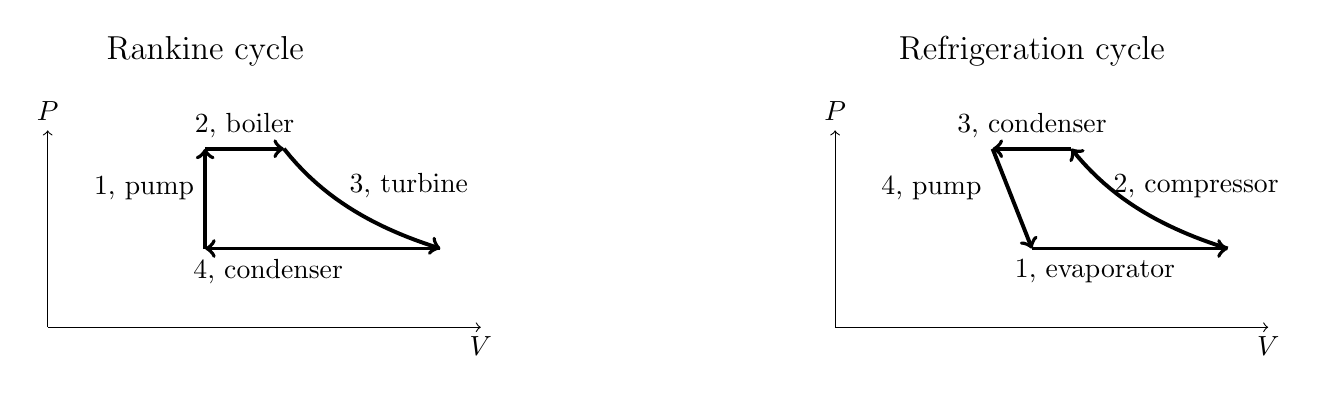
\begin{tikzpicture} %[x=8cm, y=4cm]
\draw [->] (-0.5, -0.0) -- (5.0,-0.0) node[below]{$V$};
\draw [->] (-0.5, -0.0) -- (-0.5, 2.5)  node[above]{$P$};
\draw [->, line width=0.05cm]  (1.5,1.000) -- (1.5,2.267)  node[left,  yshift=-0.5cm]                                 {1, pump};
\draw [->, line width=0.05cm]  (1.5,2.267) -- (2.5,2.267)  node[above, xshift=-0.5cm]                               {2, boiler};
\draw [->, line width=0.05cm,domain=2.5:4.486]  plot(\x, {8.176/((\x)^(1.4))}) node[above, xshift=-0.4cm, yshift=0.5cm] {3, turbine};
\draw [->, line width=0.05cm] (4.486,1.000) -- (1.5,1.000)  node[below, xshift=0.8cm]                               {4, condenser};
\node  at (1.5, 3.5) {\large Rankine cycle};

\draw [->] (9.5, -0.0) -- (15.0,-0.0) node[below]{$V$};
\draw [->] (9.5, -0.0) -- (9.5, 2.5)  node[above]{$P$};
\draw [<-, line width=0.05cm]  (12.0,1.000) -- (11.5,2.267)  node[left,  yshift=-0.5cm]                                 {4, pump};
\draw [<-, line width=0.05cm]  (11.5,2.267) -- (12.5,2.267)  node[above, xshift=-0.5cm]                                 {3, condenser};
\draw [<-, line width=0.05cm,domain=12.5:14.486]  plot(\x, {8.176/((\x-10)^(1.4))}) node[above, xshift=-0.4cm, yshift=0.5cm] {2, compressor};
\draw [<-, line width=0.05cm] (14.486,1.000) -- (12.0,1.000)  node[below, xshift=0.8cm]                               {1, evaporator};
\node at (12.0, 3.5) {\large Refrigeration cycle};
\end{tikzpicture}
\caption{The Rankine cycle and Refrigeration cycle.}
\end{figure}

\begin{equation}
e = 1-\frac{Q_c}{Q_h} = 1-\frac{H_4-H_1}{H_3-H_2} = 1-\frac{H_4-H_1}{H_3-H_1}
\end{equation}

\begin{equation}
\text{COP} = \frac{Q_c}{Q_h-Q_c} = \frac{H_1-H_4}{H_2-H_3-H_1+H_4} 
\end{equation}

\section{Homework}
Problem 4.18, 4.21, 4.26, 4.27, 4.36


